\documentclass[a4paper]{letter}
\usepackage{ngerman}
\usepackage{graphicx}
\begin{document}
\address{IONOS SE \\ Hinterm Hauptbahnhof 5 \\ 76137 Karlsruhe}
\begin{letter}{ESOC \\ Robert-Bosch-Straße 5 \\ 64293 Darmstadt}
\signature{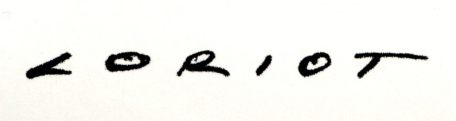
\includegraphics[width=.5\textwidth]{demos/loriot.jpg} \\ Loriot (Vicco von Bülow)}
\opening{Sehr geehrte Damen, sehr geehrte Herren,}

Ich bin tief beeindruckt von der Tatsache, dass es einer Hündin gelungen ist, in das Universum vorzustoßen, weil ich selbst zwei Hunde besitze, die in solchen Dingen gar keinen Ehrgeiz zeigen.  \\
Schon bei flüchtigem Nachdenken sind mir verschiedene Persönlichkeiten eingefallen, die ich mit größtem Vergnügen im Abstand von 1500 Kilometern um den Erdball rotieren sähe und deren Flugbahn gewiss auch viele andere Menschen mit freudigem Interesse verfolgen würden, ohne durch das Problem der gesicherten Rückkehr sonderlich erregt zu sein. – An welche Stelle kann ich diesbezügliche personelle Vorschläge richten, die \emph{vertraulich} behandelt werden?

\closing{Hochachtungsvoll,}
\end{letter}
\end{document}